\usetikzlibrary{calc}
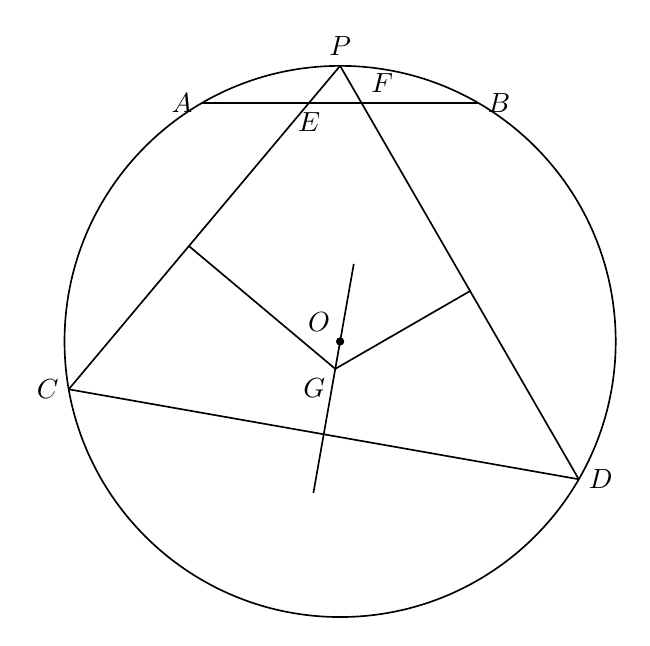
\begin{tikzpicture}[x=1cm,y=1cm,line width=.6pt,font=\normalsize]
\coordinate (O) at (0,0);
\coordinate (P) at (0,3.5);
\coordinate (A) at (-1.75,3.0311);
\coordinate (B) at (1.75,3.0311);
\coordinate (C) at (-3.4468,-0.6078);
\coordinate (D) at (3.0311,-1.75);
\coordinate (E) at (-0.3935,3.0311);
\coordinate (F) at (0.2707,3.0311);
\coordinate (G) at (-0.0614,-0.348);
\coordinate (H1) at (-1.9201,1.2117);
\coordinate (H2) at (1.6509,0.6405);
\coordinate (Qtop) at (0.1736,0.9848);
\coordinate (Qbot) at (-0.3392,-1.9237);
\draw (O) circle[radius=3.5cm];
\draw (A)--(B);
\draw (P)--(C);
\draw (P)--(D);
\draw (C)--(D);
\draw (G)--(H1);
\draw (G)--(H2);
\draw (Qtop)--(Qbot);
\fill (O) circle (1.5pt);
\node[above] at (P) {$P$};
\node[left] at (A) {$A$};
\node[right] at (B) {$B$};
\node[left] at (C) {$C$};
\node[right] at (D) {$D$};
\node[below] at (E) {$E$};
\node[above right] at (F) {$F$};
\node[above left] at (O) {$O$};
\node[below left] at (G) {$G$};
\end{tikzpicture}
